\documentclass{article}
\usepackage{graphicx}
\usepackage[utf8]{inputenc}
\usepackage[vmargin=2.5cm,hmargin=2.5cm]{geometry}
\usepackage{hyperref}

\title{Analysing Compositional Data using pyrolite }
\author{Abinu Ajithan Jyothini}
\date{August 6th 2020}
\begin{document}

\maketitle

\begin{abstract}
pyrolite, a python package used for working with geochemical data is used for analysing a general compositional dataset.It works well with a non geochemical dataset as well and i propose the usage of pyrolite's compositional data plotting for any other appropriately formatted compositional datasets. 
\end{abstract}

\section{Introduction}

pyrolite is a Python package very useful for  working with geochemical data, particularly focused on rock and mineral chemistry. pyrolite provides variety of tools for processing, transforming and visualizing geochemical data from common tabular formats.Although the python package is developed for dealing with geochemical data, it can be adapted for plotting any compositional datasets. This project makes use of the ploting tools of pyrolite for analysing Muncipal Solid Waste compositional data adapted from Yang et al\cite{yang2018comparison}.

\section{Results}
\begin{figure}
    \centering
    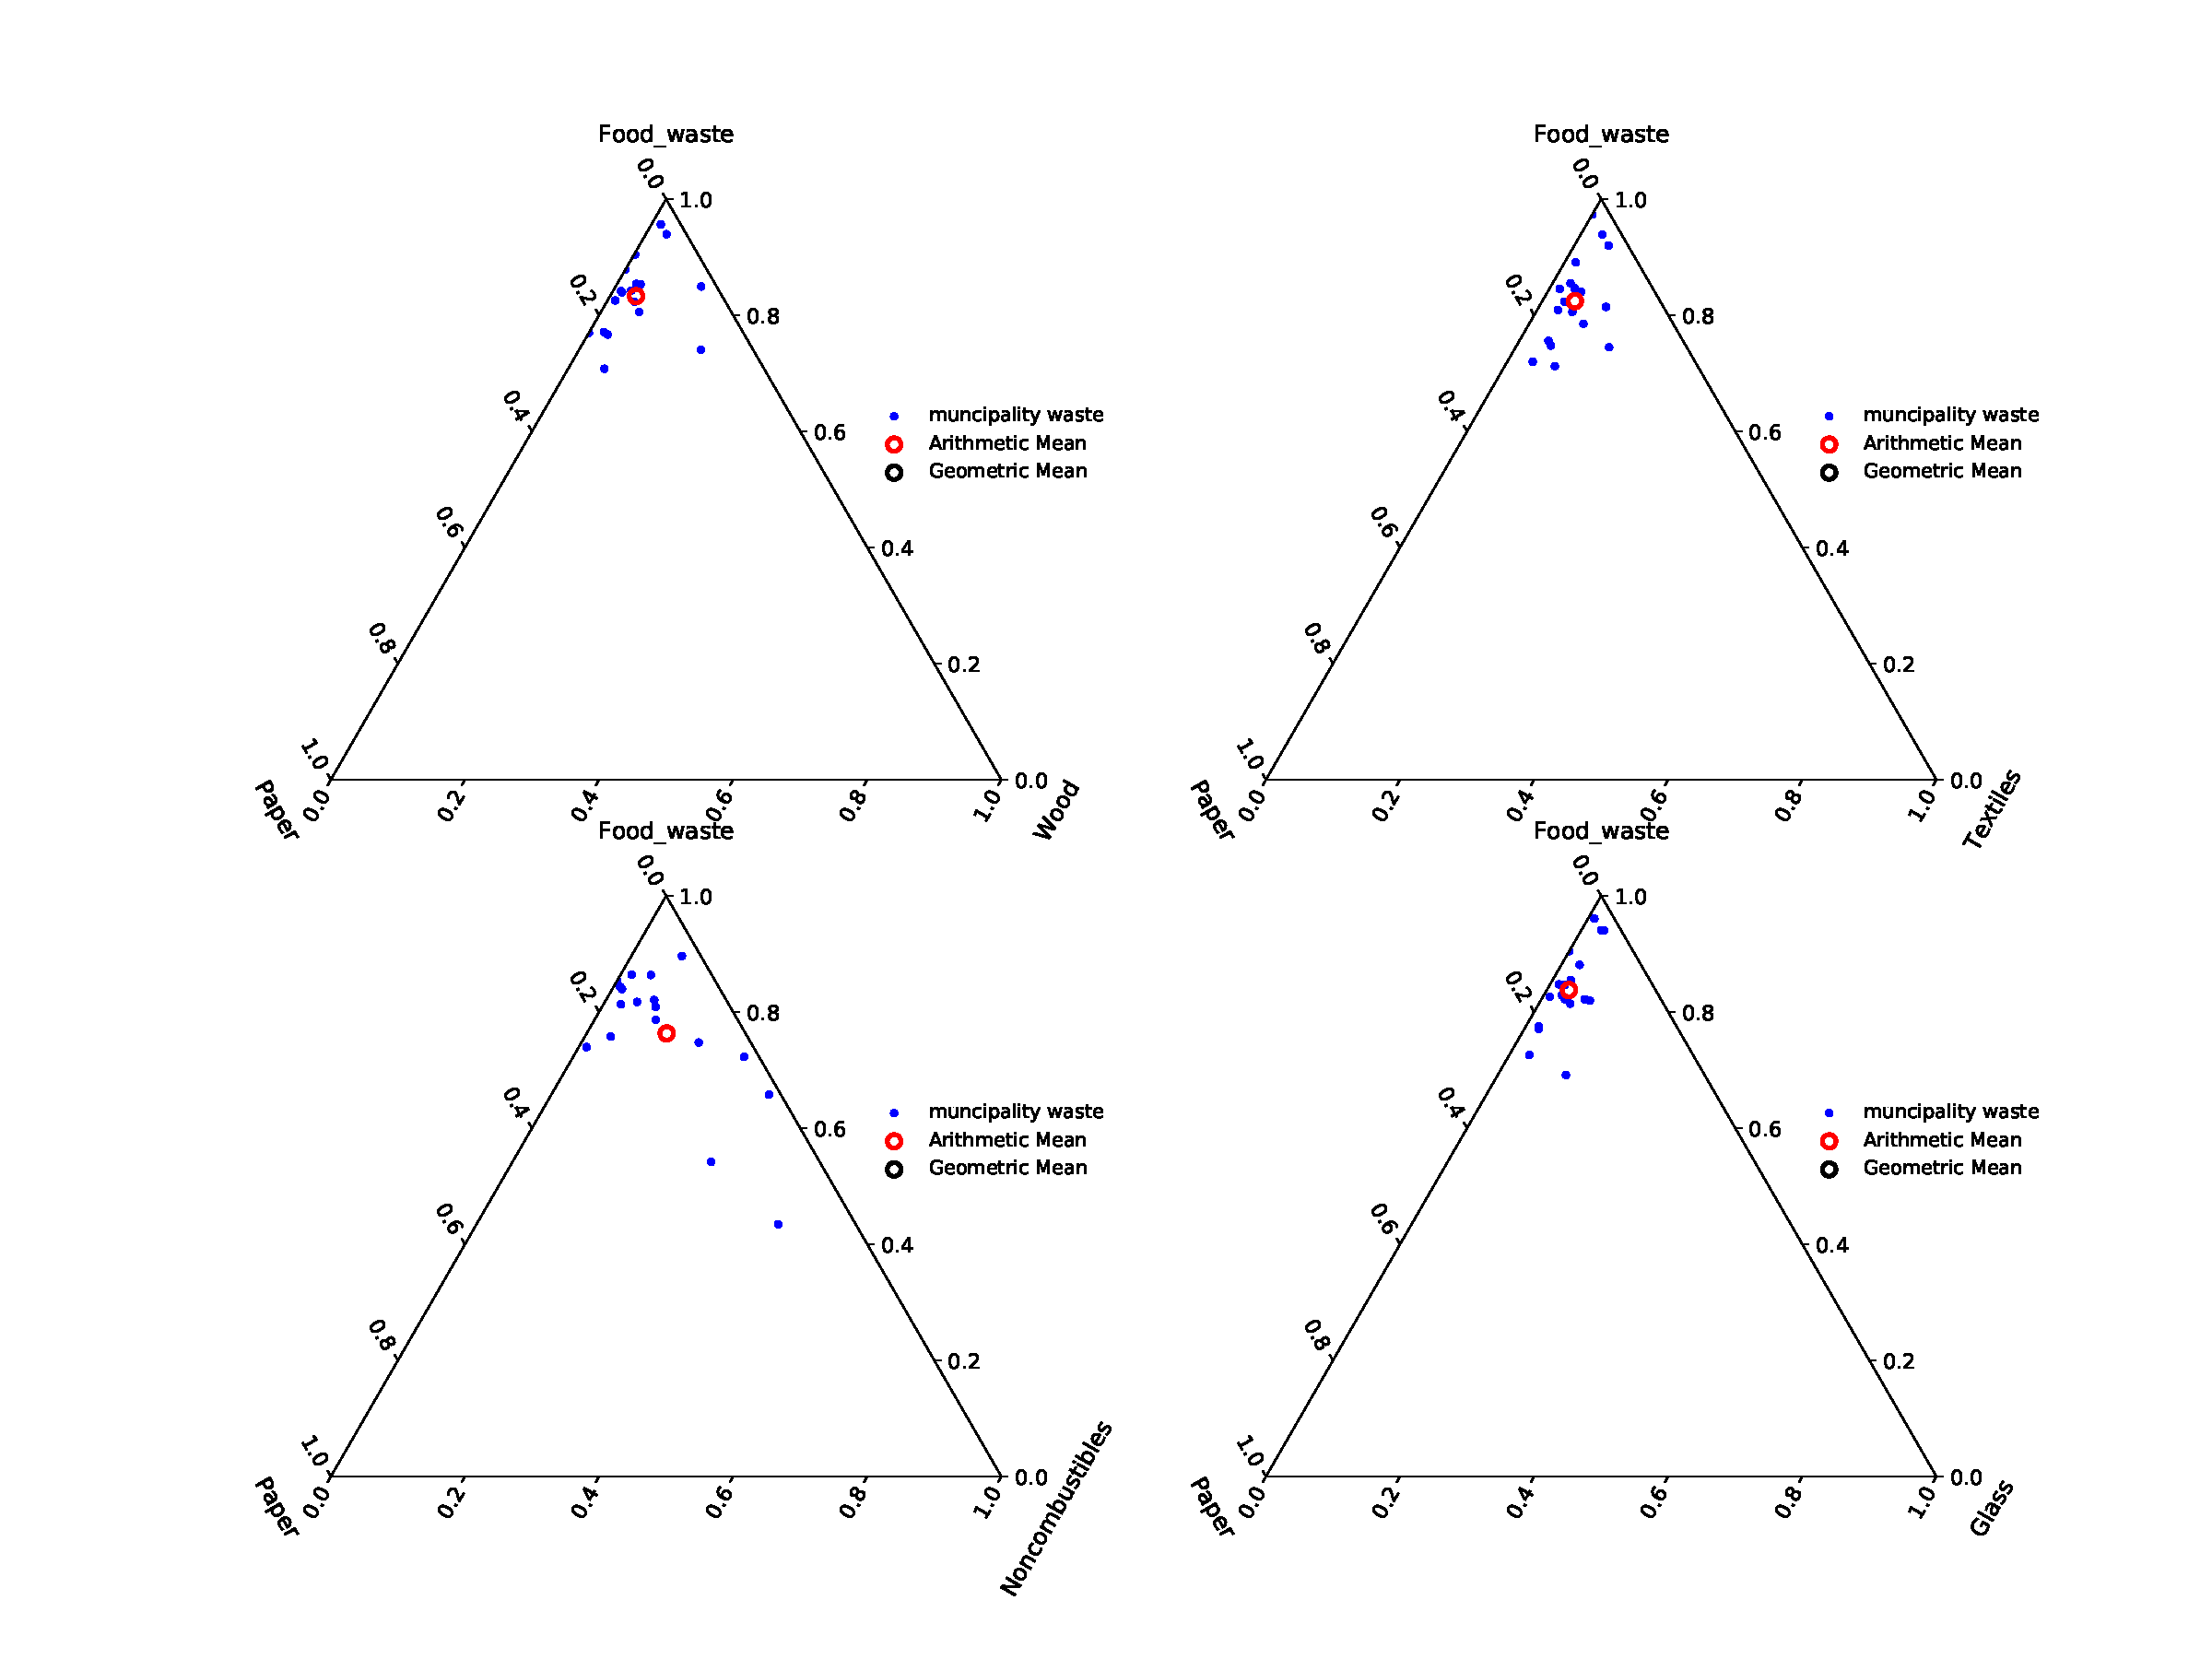
\includegraphics[width=0.9\textwidth]{ternary.png}
    \caption{Caption}
    \label{ternary}
\end{figure}

\begin{figure}
    \centering
    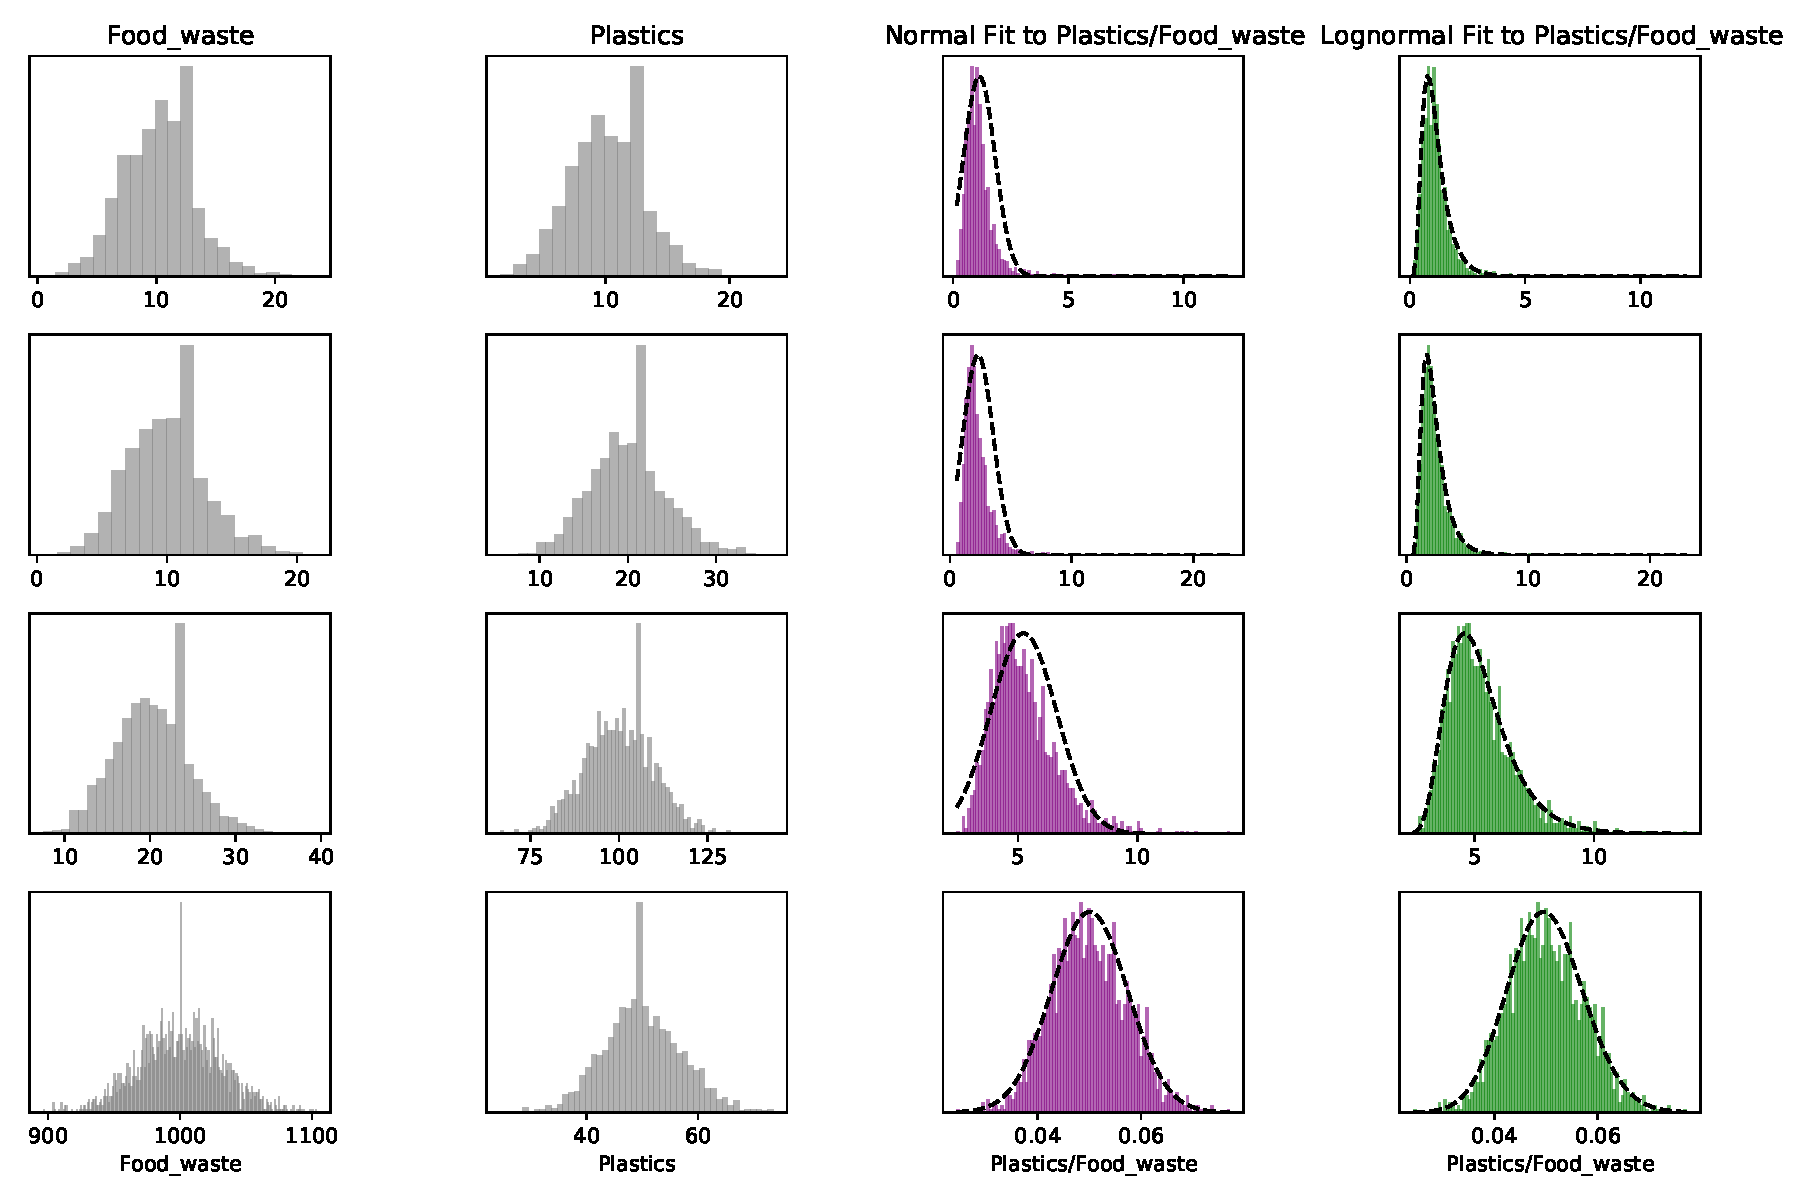
\includegraphics[width=0.9\textwidth]{lognormal.png}
    \caption{Caption}
    \label{ternary}
\end{figure}



\bibliography{rsc} 
\bibliographystyle{rsc}
\end{document}
